
\section{Глава 1. Обзор предметной области}

\subsection{Полетный контроллер}
\subsubsection{Семейства прошивок полетного контроллера}
Для получения данных с датчиков, обмена данными с периферией и управления моторной группой полетному контроллеру необходима прошивка.

Ввиду того, что нам может потребоваться доработка функционала прошивки полетного контроллера, мы не будем рассматривать прошивки с закрытым исходным кодом. Наряду с функционалом прошивки одним из ключевых факторов ее выбора будет тип открытой лицензии.

В семействе полетных контроллеров PixHawk наиболее популярны прошивки PX4 и Ardupilot. Эти прошивки активно используются как хоббистами, так и для решения профессиональных задач в промышленности и сфере эксплуатации БАС. Практически весь их функционал нацелен на выполнение автономных миссий. Ardupilot, в основном, разрабатывается и используется хоббийным сообществом. PX4 изначально был студенческой учебно-исследовательской работой, но сейчас его используют исследователи в области программирования, стабилизации и навигации БПЛА во всем мире.

Изначально это был студенческий НИР, но спустя 3 года вышел официальный релиз, сейчас его используют исследователи в области программирования, стабилизации и навигации БПЛА во всем мире. Главными особенностями PX4 являются поддержка огромного количества датчиков и навигация в режиме OFFBOARD, который позволяет управлять беспилотником при помощи бортового компьютера. OFFBOARD режим PX4 предоставляет огромные возможности для конфигурирования и управления полетным заданием с внешнего устройства, что подходит для поставленной задачи. Рассмотрим PX4 подробнее.

\subsubsection{PX4}
%\url{https://docs.px4.io/master/en/getting_started/px4_basic_concepts.html}
%\url{https://docs.px4.io/master/en/contribute/licenses.html}
%https://docs.px4.io/master/en/simulation/#simulator-mavlink-api

PX4 - прошивка с открытым исходным кодом, публикуемая под лицензией BSD-3-Clause. PX4 позволяет управлять различными типами беспилотников, включая: летательные (мультикоптеры, самолеты и вертолеты), наземные и подводные аппараты. Он совместим с большим количеством оборудования, датчиков и другой периферии. Позволяет реализовать гибкие режимы полета и функции безопасности.
Параметры PX4 настраиваются с помощью Q\-Ground\-Control \cite{px4}.

QGroundControl - кросплатформенный конфигуратор для настройки PX4 и Ardupilot прошивок. Он обеспечивает полное управление полетом и настройку беспилотника \cite{qgroundcontrol}.

PX4 для определения состояния аппарата, его стабилизации и автономного полета использует датчики, такие как: гироскоп, акселерометр, магнитометр (компас) и барометр. Для включения всех автоматических режимов и некоторых вспомогательных требуется GPS или другая система позиционирования.
Для передачи данных / телеметрии между наземной станцией управления, такой как Q\-Ground\-Control, и беспилотником, работающим под управлением PX4 может использоваться как проводное, так и беспроводное соединение по протоколу MAVLink. Он позволяет настраивать параметры во время полета, проверять телеметрию в режиме реального времени, менять миссию на лету и т. д.

PX4 можно управлять с отдельного компьютера через кабель или Wi-Fi. Дрон и компьютер обычно обмениваются данными с помощью API MAVLink, такого как MAVSDK или MAVROS \cite{px4}.

\subsubsection{MAVLink}

%\url{https://mavlink.io/en/}

MAVLink -- это протокол двоичной телеметрии, разработанный для систем с ограниченными ресурсами и каналов с ограниченной пропускной способностью. MAVLink был впервые выпущен в начале 2009 года Лоренцем Мейером (основателем PX4) и в настоящее время имеет значительное количество разработчиков. Протокол развернут в двух основных версиях: v1.0 и v2.0, которые имеют обратную совместимость (реализации v2.0 могут анализировать и отправлять пакеты v1.0).

MAVLink реализует гибрид шаблонов проектирования взаимодействия «публикация -- подписка» и «точка -- точка». В этом гибридном шаблоне потоки данных отправляются / публикуются как темы, а подпротоколы конфигурации, такие как протокол задания или протокол параметров, реализуются шаблоном «точка-точка» с повторной передачей.

Сообщения определяются в файлах XML. Каждый файл XML определяет набор сообщений, поддерживаемый MAVLink системой, также называемый «диалектом». Набор эталонных сообщений, который реализуется большинством наземных станций управления и автопилотов, определен в common.xml (большинство диалектов основано на этом определении).

Набор инструментов MAVLink использует определения XML сообщений для генерации библиотеки MAVLink для каждого из поддерживаемых языков программирования . Дроны, наземные станции управления и другие системы MAVLink используют сгенерированные библиотеки для связи. Они распространяются под лицензией MIT и поэтому могут использоваться без ограничений в любом приложении с закрытым исходным кодом без публикации исходного кода. MAVLink был впервые выпущен в начале 2009 года Лоренцем Мейером (основателем PX4) и в настоящее время имеет значительное количество разработчиков \cite{px}.

MAVLink поддерживает множество языков программирования, работающих на множестве микроконтроллеров / операционных систем (включая ARM7, ATMega, dsPic, STM32 и Windows, Linux, MacOS, Android и iOS). Допускает одновременно до 255 систем в сети (беспилотники, наземные станции и т. д.)

Обеспечивает как внешнюю, так и бортовую связь (например, между q\-ground\-con\-trol и дроном, а также между автопилотом дрона и камерой дрона с поддержкой MAVLink) \cite{mavlink}.

MAVLink развернут в двух основных версиях: v1.0 и v2.0, которые имеют обратную совместимость (реализации v2.0 могут анализировать и отправлять пакеты v1.0). Потоки телеметрических данных отправляются в многоадресном режиме, в то время как аспекты протокола, которые изменяют конфигурацию системы и требуют гарантированной доставки, являются point-to-point с повторной передачей.

%//переделать

Для того, чтобы запускать на наземной станции автономные миссии для БПЛА, необходим набор инструментов, позволяющий обрабатывать MAVLink сообщения, преобразовывать показания с камеры в координаты положения квадрокоптера и отправлять управляющие команды квадрокоптеру. Для выполнения обозначенного функционала можно использовать робототехнические фреймворки. Наиболее популярным робототехническим фреймворком является ROS.
% дописать про офборд
\subsection{Robotic Operating System}
%\url{https://www.ros.org/about-ros/}

Robotic Operating System (далее ROS) -- это гибкая платформа для написания программного обеспечения для роботов; набор инструментов, библиотек и соглашений, которые призваны упростить задачу создания сложного и надежного поведения роботов на разных роботизированных платформах \cite{ros}.

Целью создания ROS является создание среды разработки, которая позволяет разработчикам ПО для роботов взаимодействовать на глобальном уровне.

ROS сосредоточена на максимизации повторного использования кода при разработке. Основные характеристики, позволяющие это реализовать:

Распределенные процессы. Структура ROS создана в виде минимальных единиц исполняемых процессов (нод), и каждый процесс выполняется изолированно. Взаимодействие разных нод происходит только на уровне обмена сообщениями.

Управление пакетами. Несколько процессов, имеющих общую задачу, объединяются в пакеты. Управление пакетами подразумевает набор утилит, позволяющих автоматически скачивать, устанавливать и удалять пакеты. Пакетный менеджер гарантирует работоспособность и целостность установленных пакетов.

Публичные репозитории и документация. Каждый доступный пакет публикуется в публичном репозитории. Документация пакетов публикуется в единой системе, которая упрощает поиск необходимых пакетов.

Единое API. При разработке программы, использующей ROS, вы получаете простое и легко встраиваемое API. При этом при использовании API нет разницы, на каком языке была написана программа.

Поддержка различных языков программирования. ROS предоставляет клиентские библиотеки для поддержки различных языков программирования. Наиболее популярны Python, C ++, а также такие языки, как Lisp, JAVA, C\#, Lua и Ruby \cite{voltbro}.

Рассмотрим концепции ROS: ноды, топики, сервисы.

\subsubsection{Ноды}
Нода представляет собой процесс, который выполняет вычисления. Ноды объединяются в граф и взаимодействуют друг с другом с помощью топиков, сервисов и сервера параметров. Ноды предназначены для работы в мелкомасштабном масштабе; система управления роботом обычно состоит из множества нод.

Все ноды имеют имя ресурса графа, которое однозначно идентифицирует их для остальной системы. Ноды также имеют типы, который упрощает процесс обращения к исполняемому файлу узла в файловой системе. Эти типы представляют собой имена ресурсов пакета с именем пакета ноды и именем исполняемого файла ноды. Чтобы определить тип ноды, ROS ищет все исполняемые файлы в пакете с указанным именем и выбирает первый из найденных \cite{ros}. 
% http://wiki.ros.org/Nodes \cite{ros}

%ROS-нода – это специальная программа (обычно написанная на Python или C++), которая взаимодействует с другими нодами посредством ROS-топиков и ROS-сервисов. Разделение сложных робототехнических систем на изолированные ноды дает определенные преимущества: понижается связанность кода, повышается переиспользуемость и надежность.

Очень многие робототехнические библиотеки и драйвера выполнены в виде ROS-нод.
Для того, чтобы преобразовать обычную программу в ROS-ноду, необходимо подключить к ней библиотеку rospy или roscpp и добавить инициализирующий код.

Пример ROS-ноды на языке Python:

\begin{Program}[H]
	\caption{Пример ROS-ноды на языке Python} \label{lst:1}
\begin{MyCode}
import rospy
		
rospy.init_node('my_ros_node')  # имя ROS-ноды
		
rospy.spin()  # входим в бесконечный цикл...
\end{MyCode}
\end{Program}

Возможность запуска нескольких нод в одном процессе осуществляет пакет nodelet. Он позволяет производить обмен сообщений внутри процесса без затрат на копирование \cite{ros}.
%http://wiki.ros.org/nodelet

\subsubsection{Топики}
Топиками называют шины, по которым ноды обмениваются сообщениями. Топики имеют семантику анонимной публикации/подписки, которая отделяет производство информации от ее потребления. Как правило, ноды не знают, с кем они общаются. Вместо этого ноды, которые заинтересованы в данных, подписываются на соответствующие топики; ноды, которые генерируют данные, публикуются в соответствующем топике. У топиков может быть несколько издателей и подписчиков.

Топики предназначены для однонаправленного потокового общения.

Каждый топик строго типизирован в соответствии с типом сообщения ROS, используемым для публикации в ней, и ноды могут получать сообщения только с совпадающим типом. Master не обеспечивает согласованность типа среди издателей, но абоненты не будут устанавливать сообщение транспорта, если топики не совпадают. Кроме того, все клиенты ROS проверяют совпадение MD5, вычисленного из файлов msg. Эта проверка гарантирует, что ноды ROS были скомпилированы из согласованных кодовых баз \cite{ros}.
% http://wiki.ros.org/Topics

\begin{Program}[H]
	\caption{Пример публикации сообщения типа строка в топик foo на языке Python} \label{lst:2}
\begin{MyCode}
from std_msgs.msg import String
		
# создаем Publisher'а
foo_pub = rospy.Publisher('/foo', String, queue_size=1)
		
# публикуем сообщение
foo_pub.publish(data='Hello, world!')
\end{MyCode}
\end{Program}

\begin{Program}[H]
	\caption{Пример подписки на топик /foo на языке Python} \label{lst:3}
\begin{MyCode}
def foo_callback(msg):
print msg.data
		
#При получении сообщения в топик /foo
#будет вызвана функция foo_callback.
rospy.Subscriber('/foo', String, foo_callback)
\end{MyCode}
\end{Program}

Также существует возможность работы с топиками с помощью утилиты rostopic. Например, с помощью следующей команды можно просматривать сообщения, публикуемые в топик /mavros/state:
$ rostopic echo /mavros/state
\subsubsection{Сервисы}

Сервис -- это некоторый аналог функции, которая может быть вызвана из одной ноды, а обработана в другой. У сервиса есть имя, аналогичное имени топика, и 2 типа сообщений: тип запроса и тип ответа \cite{clover}.

\begin{Program}[H]
	\caption{Пример вызова ROS-сервиса из языка Python} \label{lst:4}
\begin{MyCode}
from clover.srv import GetTelemetry

# Создаем обертку над сервисом get_telemetry
# пакета clover с типом GetTelemetry:

get_telemetry = rospy.ServiceProxy('get_telemetry', srv.GetTelemetry)
		
# Вызываем сервис и получаем телеметрию квадрокоптера:

telemetry = get_telemetry()

# С сервисами можно также работать при помощи утилиты rosservice.
# Так можно вызвать сервис /get_telemetry из командной строки:
		
rosservice call /get_telemetry "{frame_id: ''}"
\end{MyCode}
\end{Program}

\subsubsection{MAVROS}
%\url{https://clover.coex.tech/ru/mavros.html}
%\url{https://dev.px4.io/master/en/ros/mavros\_installation.html}
Так как мы выбрали ROS как основной фреймворк для реализации нашего решения и MAVLink, в качестве основного протокола -- нам необходим компонент, обеспечивающий взаимодействие обозначенных систем.
MAVROS (MAVLink + ROS) -- это пакет для ROS, предоставляющий возможность управлять беспилотниками по протоколу MAVLink. MAVROS поддерживает полетные стеки PX4 и APM. Связь организовывается по UART, USB, TCP или UDP.

MAVROS подписывается на определенные ROS-топики в ожидании команд, публикует в другие топики телеметрию, и предоставляет сервисы.
Пакет mavros обеспечивает расширяемую связь MAVLink между компьютерами, на которых работает ROS, автопилоты с поддержкой MAVLink и GCS с поддержкой MAVLink. Нода MAVROS запускается в launch-файле \cite{clover}.

Прошивка рх4 позволяет использовать внешние системы видеонавигации, рассмотрим подробнее некоторые из них.
%MAVROS -- это «официальный» поддерживаемый мост между ROS и протоколом MAVLink. В настоящее время он расширяется, чтобы включить обмен сообщениями fast-RTPS, включая уровень для преобразования сообщений uORB PX4 в общие идиомы ROS. Эти расширения в последующем могут существенно улучшить скорость работы разрабатываемого решения.
%https://dev.px4.io/v1.9.0/en/setup/fast-rtps-installation.html доработать
\subsection{Потоковая передача видео}

\subsubsection{GStreamer}

GStreamer -- это библиотека для построения графиков компонентов обработки мультимедиа. Он поддерживается различными мультимедийными приложениями, позволяет осуществлять потоковую передачу аудио / видео и обрабатывать звук / видео. GStreamer является свободным программным обеспечением с лицензией GNU LGPL.

Практически все в GStreamer является элементом. Все, начиная от обычных источников потоков (filesrc, alsasrc, и т. п.), обработчиков потоков (демультиплексоры, декодеры, фильтры, и т. п.) и заканчивая конечными устройствами вывода (alsasink, fakesink, filesink, и т. п.).

Pad — это некая точка подключения одного элемента к другому, если более просто — это входы и выходы элемента (рис. \ref{fig:ris1}). Обычно они именуются «sink» — вход и «src» — выход.
% ~\ref{fig:ris1}
\begin{figure}[H]
	\centering
	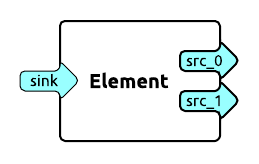
\includegraphics[width=0.5\linewidth]{pics/pic1}
	\caption{ GStreamer pads (sink, src\_0, src\_1)
	}
	\label{fig:ris1}
\end{figure}
Жизненный цикл элементы проводят внутри контейнеров. Контейнер управляет рассылкой сообщений от элемента к элементу, статусами элементов. Контейнеры делятся на два вида: Bin и Pipeline.

Bin -- простой контейнер, который управляет рассылкой сообщений от элемента к элементу которые находятся внутри него. Bin обычно используется для создания группы элементов которые должны совершать какое-либо действие. 
Pipeline является контейнером верхнего уровня, он управляет синхронизацией элементов, рассылает статусы. Например, если pipeline установить статус PAUSED, этот статус будет автоматически разослан всем элементам которые находятся внутри него. Pipeline является реализацией Bin \cite{gstreamer}. 

Источники данных -- это класс плагинов GStreamer, который позволяет читать медиаданные из различных источников, таких как файловая система или аудио-входы звуковой карты. Также, они позволяют получать медиапоток с различных серверов потокового вещания, таких как HTTP (ICECast, ShoutCast), RTSP, RTMP, TCP и UDP. 

Утилита gst-launch-1.0 позволяет запускать GStreamer pipeline без написания кода. Запуск pipeline имеет следующий вид:
gst-launch-1.0 описание-pipeline

Описание pipeline, в свою очередь, делится на описание элементов вида:
element1 property1=value1 property2=value2 ! element2.

Есть элемент типа element1 со свойствами property1 и property2, которые имеют значения value1 и value2 соответственно, и есть элемент типа element2. Символ «!» указывает на то, что выход element1 необходимо соединить с входом element2.
%https://habr.com/ru/post/179167/
% https://docs.gstreamer.com/documentation/
В случае с Raspberry источником видеопотока (element1) является rpicamsrc, который захватывает изображение с RPi камеры. rpicamsrc может выводить видео в виде необработанных кадров или закодированное в формате (M)JPEG или H.264 \cite{gstreamer1}. В качестве element2 будет выступать устройство вывода udpsink,-- это сетевой приемник, который отправляет UDP-пакеты в сеть.
%https://gstreamer.freedesktop.org/documentation/udp/udpsink.html
Для приема и обработки видеопотока на наземной станции может быть использован gscam.

\subsubsection{gscam}
gscam -- ROS драйвер, изначально разработанный для трансляции видеопотока на основе gstreamer через стандартный API камеры ROS. Его можно установить из стандартных репозиториев, предоставляемых менеджером apt или собрать вручную с помощью catkin\_make. gscam может быть запущен и как нода, и как нодлет.

gscam может подключаться к специально отформатированному конвейеру. При условии, что этот конвейер обрабатывает видео в формате RGB. gscam ожидает, что переменная окружения GSCAM\_CONFIG будет содержать gstreamer определение конвейера для его запуска.
gscam получает стрим и публикует 2 топика: /camera/image\_raw(необработанное изображение) и /camera/camera\_info(содержит калибровку камеры и дополнительные данные о конфигурации камеры) \cite{ros}.
% http://wiki.ros.org/gscam

\subsubsection{aruco\_gridboard}
Нода aruco\_gridboard подписывается на топики, публикуемые gscam: топик изображения /camera/image и топик /camera/camera\_info, содержащий параметры камеры. При получении видеопотока aruco\_gridboard распознает карту aruco маркеров, описанную в файле yaml, и публикует статус в топик /vision/status, а полученные координаты в /vision/pose.

Таким образом, видео с Raspberry Pi c помощью gstreamer передается по UDP на ip-адрес наземной станции; нода gscam получает UDP-пакеты и публикует изображение в топики /camera/image\_raw и /camera/camera\_info; aruco\_gridboard подписывается на топики с изображением и информацией о камере и публикует сообщения о положении дрона относительно карты маркеров в /mavros/vision\_pose/pose топик.

%http://www.uco.es/investiga/grupos/ava/sites/default/files/GarridoJurado2014.pdf
